% Chapter 1

\chapter{Introducción general} % Main chapter title

\label{Chapter1} % For referencing the chapter elsewhere, use \ref{Chapter1} 
\label{IntroGeneral}
En este capítulo se presentan las características de los robots de servicio, se  reseña el uso de luz ultravioleta como germicida y se exponen los objetivos que motivaron el presente trabajo y sus respectivo alcance.
%----------------------------------------------------------------------------------------

% Define some commands to keep the formatting separated from the content 
\newcommand{\keyword}[1]{\textbf{#1}}
\newcommand{\tabhead}[1]{\textbf{#1}}
\newcommand{\code}[1]{\texttt{#1}}
\newcommand{\file}[1]{\texttt{\bfseries#1}}
\newcommand{\option}[1]{\texttt{\itshape#1}}
\newcommand{\grados}{$^{\circ}$}

%----------------------------------------------------------------------------------------

%\section{Introducción}

%----------------------------------------------------------------------------------------
\section{Robots de servicio}

A lo largo del siglo XX la robótica pasó de ser una temática de la rama de la ciencia ficción, a cumplir un importante rol dentro de los complejos industriales. En los últimos años los robots han pasado a tener cada vez más tareas de “servicio” para ambientes  públicos y hogareños.
La robótica de servicios abarca un amplio campo de aplicaciones, la mayoría de las cuales tienen diferentes grados de automatización, desde la teleoperación completa hasta el funcionamiento autónomo, y constituye un campo de aplicación más diverso que el de la robótica industrial. En la  figura \ref{fig:robotsservicio} se pueden observar tres tipos de robots de servicios: una aspiradora hogareña, un cortador de césped y un limpiavidrios.

\begin{figure}[h]
	\centering
	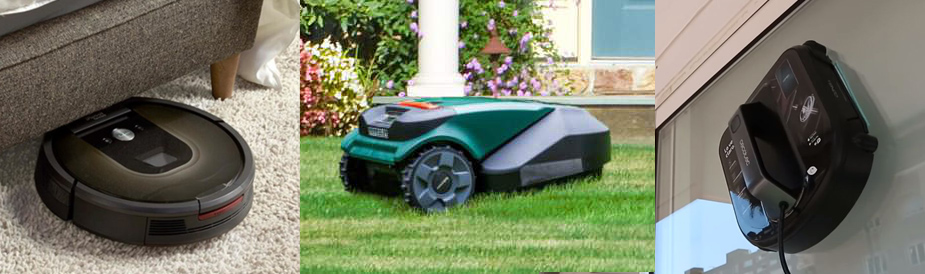
\includegraphics[width=\textwidth]{./Figures/robotsservicio.jpg}
	\caption{Robots de servicio\protect\footnotemark.}
	\label{fig:robotsservicio}
\end{figure}
\footnotetext{Imágenes tomadas de \url{https://www.domotizar.com/}}


A mediados de la década de 1990, la Comisión Económica de las Naciones Unidas para Europa (UNECE) \citep{UNECE} y la Federación Internacional de Robótica (IFR) \citep{IFR} adoptaron un sistema de clasificación de robots de servicio dividida por categorías y tipos de interacción, que se ha mantenido hasta la actualidad. En la  figura \ref{fig:robotsservicio} se puede observar los primeros ítems de clasificación para robots domésticos/personales de acuerdo a los tipos y áreas de aplicación.
\pagebreak


\begin{figure}[h]
	\centering
	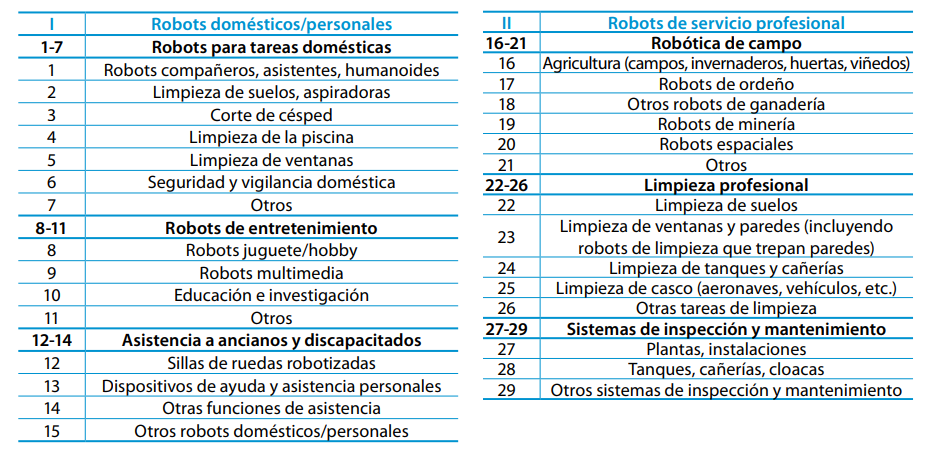
\includegraphics[width=\textwidth]{./Figures/clasificacion.png}
	\caption{Clasificación de robots de servicio\protect\footnotemark.}
	\label{fig:clasificacion}
\end{figure}
\footnotetext{Imagen tomada de \url{https://www.editores-srl.com.ar/sites/default/files/aa1_ifr_robots.pdf}}




\subsection{Robots móviles para inspección y limpieza}

Los robots móviles son dispositivos que poseen un sistema de locomoción capaz de navegar a través de un determinado ambiente de trabajo. Normalmente cuentan con cierto nivel de autonomía que les permite el desplazamiento sin colisiones por un recorrido específico. Sus aplicaciones son muchas y en general  están relacionadas con tareas monótonas o riesgosas para la salud humana.

Las plataformas móviles pueden realizar tareas de inspección y limpieza de manera autónoma o controlada remotamente por un operador. Son utilizadas en zonas de difícil acceso debido a limitaciones de espacio o razones de seguridad. Este tipo de robot suele contar con sensores de distinto tipo, para detectar los límites y obstáculos ante los que se presentan.
 
La proliferación de robots para limpieza se incrementó fuertemente a partir de la pandemia de Covid-19, con lo que se los puede encontrar hoy en día en espacios en los que antes no estaban presentes, tales como salas médicas,  hoteles y en el transporte público \citep{Cleaning}. 

Estos dispositivos “de interior” abarcan varios tipos. En la  figura \ref{fig:robotslimpieza} se puede observar un modelo de robot trapeador húmedo, una aspiradora robótica y un limpiavidrios automático, a modo de ejemplo.

\begin{figure}[h]
	\centering
	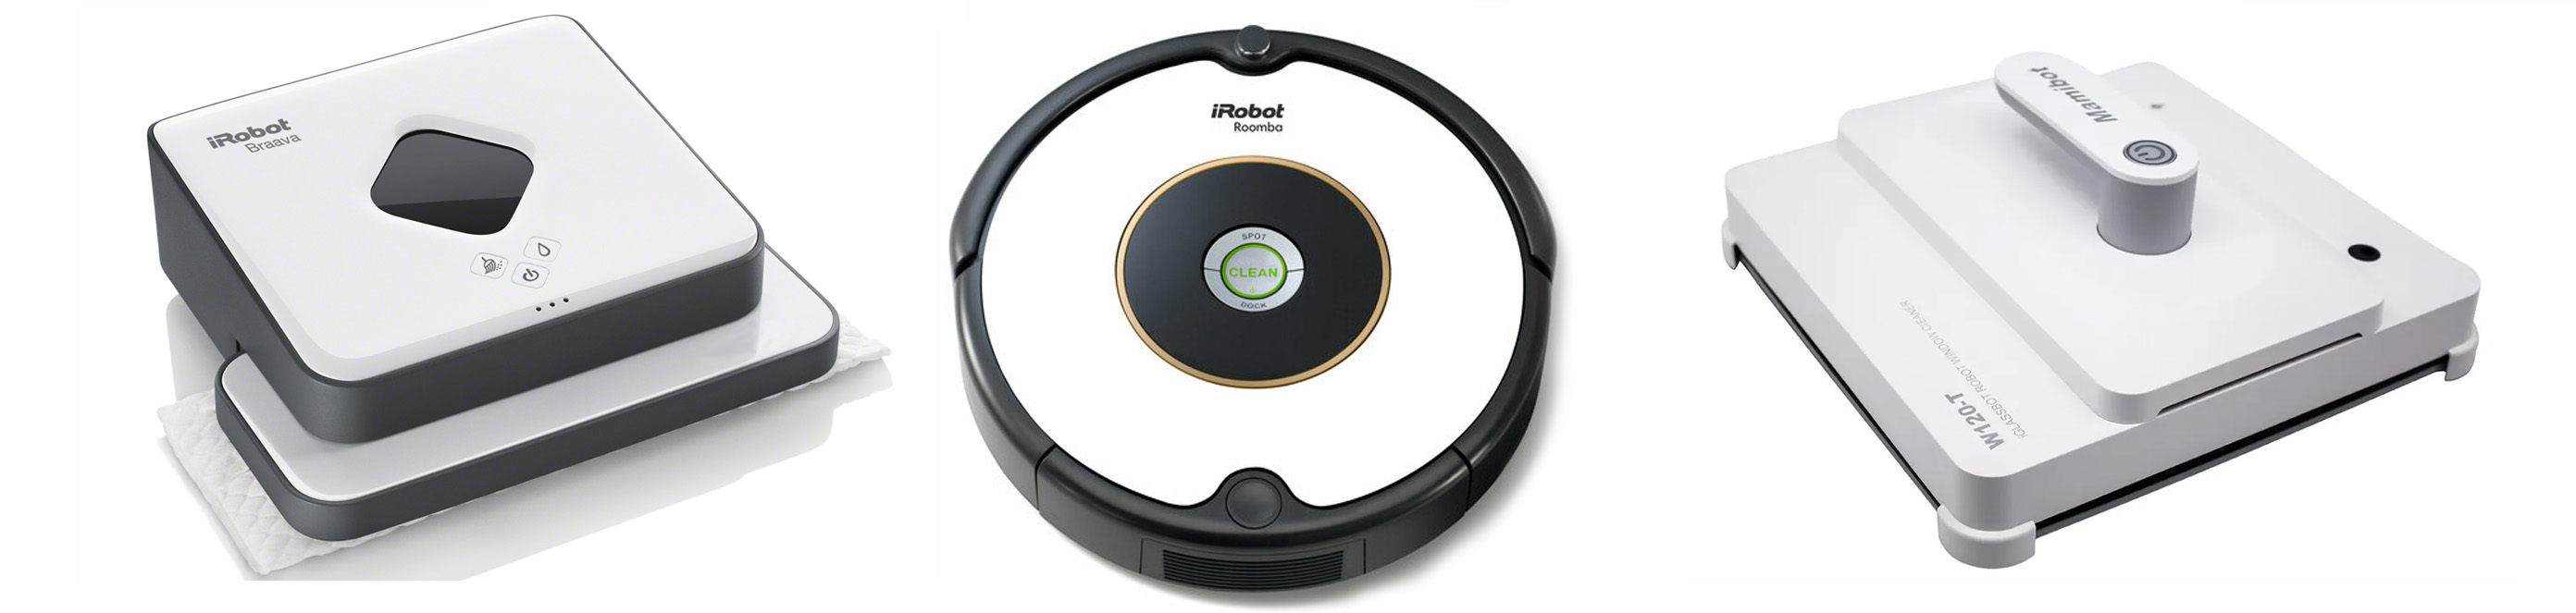
\includegraphics[width=\textwidth]{./Figures/robotslimpieza.jpg}
	\caption{Distintos tipos de robot de limpieza\protect\footnotemark.}
	\label{fig:robotslimpieza}
\end{figure}
\footnotetext{Imágenes tomadas de \url{https://www.domotizar.com/}}


%----------------------------------------------------------------------------------------

\subsection{Robots de desinfección por luz ultravioleta}

Desde hace tiempo se utiliza luz ultravioleta para la desinfección de agua potable, y más recientemente ha sido incorporada como método germicida en conductos de ventilación. También se ha utilizado para la desinfección de instrumental e insumos en ambientes hospitalarios. En el  siguiente apartado se dará referencia acerca de la eficiencia de la luz ultravioleta, dentro de cierto rango de longitud de onda, para el control de bacterias y virus.

En los últimos dos años, con el aumento de precauciones debido a la pandemia mundial por el COVID-19, comenzaron a comercializarse robots móviles de luz ultravioleta germicida, para desinfectar quirófanos y salas de hospitales. Estos robots, poseen paneles con tubos ultravioleta para poder irradiar completamente una habitación o parte de la misma y son de alturas entre los 120 y los 180 cm para poder iluminar camas y mesas desde arriba y poder pasar por puertas y aberturas convencionales. La cobertura de estos robots suele ser mayor a los 180 grados, por lo que resulta importante no solo el recorrido realizado para abarcar todas las superficies, sino también evitar la presencia cercana de personas ya que la exposición de rayos ultravioleta puede ser perjudicial para la piel y la vista. En la figura \ref{fig:robotuv} se muestra un robot de estas características. 


\begin{figure}[h]
	\centering
	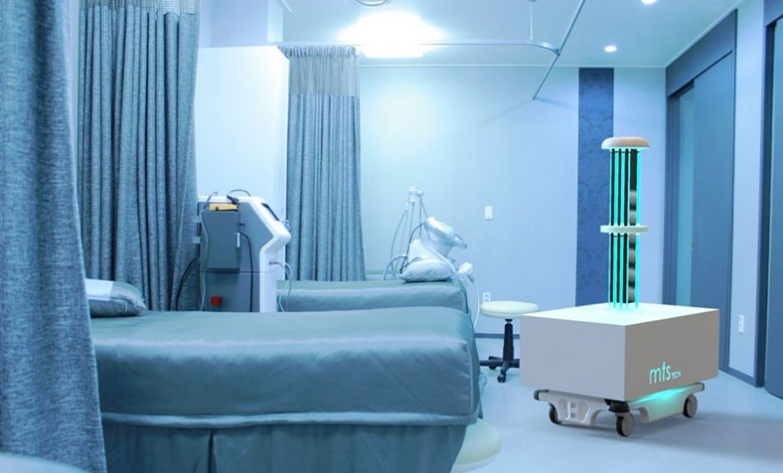
\includegraphics[width=\textwidth]{./Figures/robothospitalario.PNG}
	\caption{Robot desinfectante por luz ultravioleta en una sala de hospital\protect\footnotemark.}
	\label{fig:robotuv}
\end{figure}
\footnotetext{Imagen tomada de \url{https://www.infoplc.net/plus-plus/empresas/item/107726-mts-tech-robot-movil-ultravioleta-covid-19}}

Además de los hospitales, estos robots están siendo usados en otros espacios, como vagones del subterráneo, espacios comunes en hoteles, oficinas y áreas de control en aeropuertos \citep{masrobots}.

Otra aplicación que empieza a dársele a los robots UV-C es la desinfección fungicida en viñedos (en particular el oidio, que es un hongo que ataca todos los tejidos verdes del cultivo). Dispositivos robot recorren las plantaciones por la noche con paneles ultravioleta cuya luz daña el ADN del hongo, sin afectar a las plantas \citep{infowine}.

En 2020, la empresa argentina UV- Robotics lanzó el UVR-Robot \citep{UVR} que cuenta con tubos de luz UV-C germicida dispuestos en un arreglo de 360 grados para que la luz llegue hasta cualquier rincón y con una plataforma omnidireccional. El proceso toma  entre 5 y 15 minutos según la superficie, y se lo puede dirigir a control remoto. Esto le permite desinfectar autobuses, aviones y otros medios de transporte, salas de espera, centros de mayores, colegios, entidades bancarias, hoteles, ascensores o aseos. La iniciativa  tuvo el apoyo del Ministerio de Desarrollo Nacional y cuenta con validaciones y homologaciones de la Universidad Tecnológica Nacional. En la figura \ref{fig:uvrobot} se observa al UVR-Robot desinfectando un vagón de tren subterráneo. 

\begin{figure}[h]
	\centering
	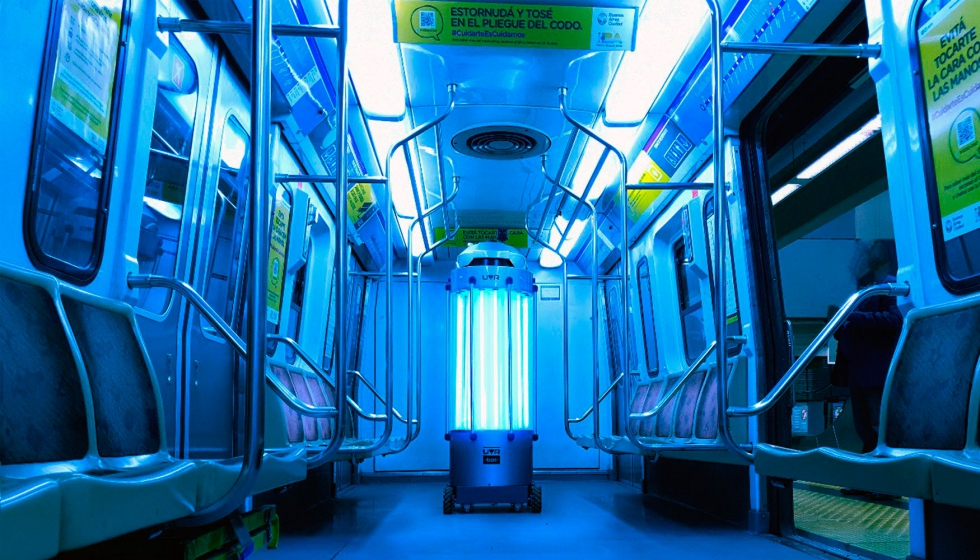
\includegraphics[width=12cm]{./Figures/uvrobot.jpeg}
	\caption{UVR-Robot de la agencia nacional UV- Robotics\protect\footnotemark.}
	\label{fig:uvrobot}
\end{figure}
\footnotetext{Imagen tomada de \url{https://www.interempresas.net/Tecnologia-aulas/Articulos/321010-UVR-bot-reto-acabar-cualquier-rastro-covid-19-20-minutos-luz-ultravioleta.html}}

A nivel hogareño, muchos robots de limpieza empiezan a incorporar la luz ultravioleta como medio de desinfección. En general, es una característica adicional que presentan las aspiradoras robóticas que además de barrido y trapeado húmedo agregan la esterilización de suelos con luz ultravioleta, resultando hoy en día una característica evaluada en las comparativas de los distintos productos  \citep{prueba}.


%----------------------------------------------------------------------------------------
\section{Desinfección usando luz ultravioleta}

El espectro ultravioleta (UV) abarca la banda de radiación electromagnética entre los 400 y 100 nm, presentando una longitud de onda menor que la de la luz visible y mayor que la de los rayos X.  Se divide en las siguientes categorías principales:

\begin{itemize}
	\item los rayos UV-A (400 – 315 nm), que son los más cercanos al espectro visible.
	\item los rayos UV-B (315 – 280 nm), que son absorbidos en gran parte por diferentes elementos a medida que atraviesan el cielo.
	\item los rayos UV-C (280 – 200 nm), que son absorbidos totalmente por la capa de ozono.
\end{itemize}


En la  figura \ref{fig:espectro} se observa detalle de parte del espectro de radiación electromagnética y su clasificación según longitud de onda.


\begin{figure}[h]
	\centering
	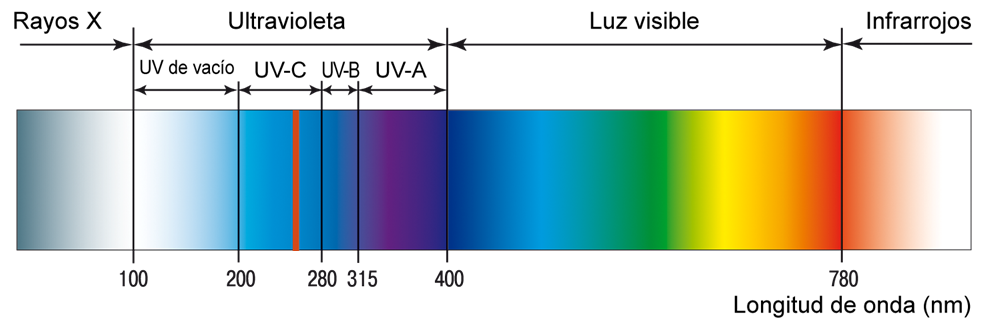
\includegraphics[width=14cm]{./Figures/espectro.PNG}
	\caption{clasificación según longitud de onda.\protect\footnotemark.}
	\label{fig:espectro}
\end{figure}
\footnotetext{Imagen tomada de \url{https://www.lit-uv.com/es/technology/}}

La utilización de luz ultravioleta UV-C como germicida ha demostrado efectividad para la esterilización  las bacterias, gérmenes, virus, algas y esporas. 

Los virus tienen un tamaño inferior a un micrómetro (µm, una millonésima parte de un metro) y las bacterias son típicamente de 0,5 a 5 µm. Técnicamente es incorrecto decir que los rayos  UV-C matan a los virus, siendo que no se trata de organismos vivientes. Sin embargo, el comité de foto-biología de la \emph{ Illuminating Engineering Society} (IES) informa que los fotones UV-C interactúan con el ARN y las moléculas de ADN en un virus o bacteria de modo que se evita su reproducción y por lo tanto su efecto infeccioso. Una célula que no puede reproducirse se considera muerta; ya que no puede multiplicarse dentro del anfitrión. A este proceso se lo denomina “desactivación”   \citep{IES}. En la figura \ref{fig:adn} se representa el efecto de la luz UV-C en el ADN de bacterias, gérmenes, virus, algas y esporas. 
 

\begin{figure}[h]
	\centering
	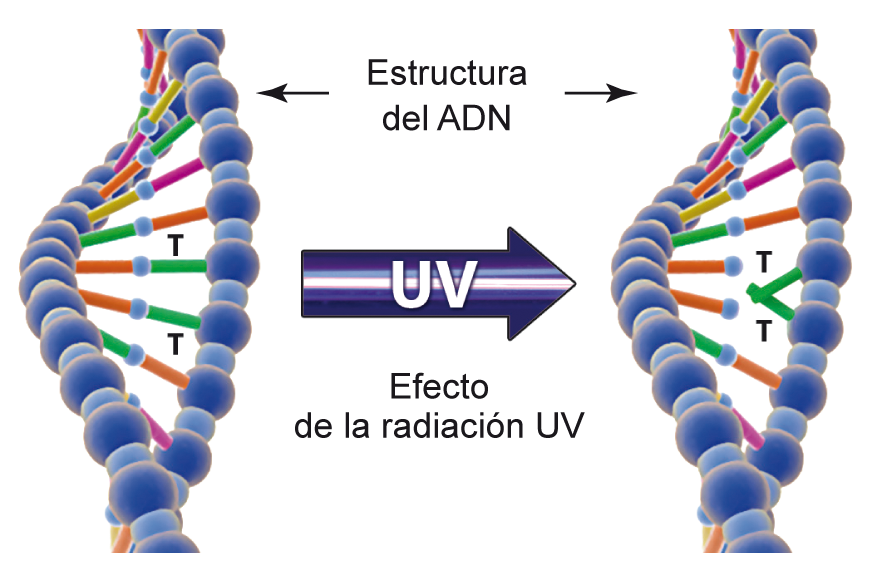
\includegraphics[width=9cm]{./Figures/adn.png}
	\caption{Efecto de la UV-C sobre el ADN de microorganismos\protect\footnotemark.}
	\label{fig:adn}
\end{figure}
\footnotetext{Imagen tomada de \url{https://www.lit-uv.com/es/technology//}}

La \emph{International Ultraviolet Association}  (IUVA) afirma que los resultados de pruebas en laboratorio de desinfección utilizando UV-C entre los 200 y 280 nm demuestran especial utilidad para reducir la transmisión de los virus causantes del COVID-19:  SARS-CoV-1 y MERS-CoV \citep{IUA}. En la práctica, el efecto depende de factores tales como  el tiempo de exposición y obstrucción que puedan tener los rayos para alcanzar plenamente los pliegues u ondulaciones que pudiera tener la superficie a desinfectar. 

En un informe sobre utilización de la radiación ultravioleta para desinfección \citep{CSIC}, el Consejo Superior de Investigaciones Científicas de España, concluye que el uso de radicación UV-C es muy adecuado para la desinfección de microorganismos y de virus, y propone su uso en combinación con métodos tradicionales para la desinfección en  zonas de alta contaminación.

Una de las ventajas de este método de desinfección radica en que una vez terminada el ambiente puede volver a ser utilizado inmediatamente, ya que no existe radiación persistente. La desinfección  por UV-C resulta además menos contaminante para el medio ambiente, al no exponer al ser humano a los riesgos derivados del uso de productos químicos. La desinfección germicida por ultravioleta es especialmente recomendada cuando debe realizarse sobre materiales que podrían verse afectados o dañados ante la limpieza continua con productos a base de químicos líquidos, como ser dispositivos electrónicos o materiales susceptibles a la  oxidación \citep{interior}. En la figura \ref{fig:gabineteuv} se muestra un gabinete utilizado para la desinfección ultravioleta de toallas, pinzas, cortauñas, limpieza de cepillos de dientes, teléfono móvil, etc.
\vspace{12mm}

\begin{figure}[h]
	\centering
	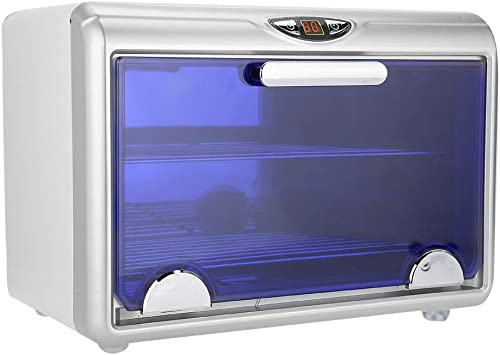
\includegraphics[width=7cm]{./Figures/gabineteuv.jpg}
	\caption{Ejemplo de gabinete de desinfección ultravioleta.}
	\label{fig:gabineteuv}
\end{figure}



La desinfección por rayos UV-C es también útil en el caso de superficies de difícil acceso por su ubicación o cuando la zona presenta formas y estructuras que no permiten la higienización por contacto con paños o rociadores. 
 
Por otra parte, si bien la Organización Mundial de la Salud (OMS) recomienda el uso de rayos UV-C para desinfección, también alerta sobre los riesgos de  exposición en seres humanos y animales, cuya piel puede verse irritada, a la vez que puede producir daños a la vista \citep{MYTH}. En este sentido promueven la limpieza de manos periódica con jabón o con alcohol, y dejan la esterilización con UV-C para  instrumental y objetos de uso diario.



%----------------------------------------------------------------------------------------

\section{Motivación}

Existen cada vez más robots de servicio orientados a tareas específicas de ayuda para la industria y el hogar. En los últimos años empezaron a proliferar los robots aspiradoras a nivel hogareño, que realizan su tarea en forma autónoma en ambientes cerrados. 
Basado en el funcionamiento de estos robots, y en un contexto mundial en el que es importante reforzar los niveles de higiene, es que surge la idea de construir una plataforma móvil de dimensiones similares, que pudiera utilizarse para desinfección por rayos UV-C. 

Si bien los robots de desinfección surgidos durante la pandemia COVID-19 son de dimensiones mucho mayores, los conceptos y criterios utilizados en el actual prototipo pueden ser aplicados a dispositivos de estas características. De hecho, se ha visto que muchos robots de limpieza hogareña empiezan a incorporar la desinfección por UV-C como parte de sus prestaciones. En un informe sobre utilización de la radiación ultravioleta para desinfección [xx] elaborado por el Consejo Superior de Investigaciones Científicas de España, se propone como algo necesario el diseño de robots móviles que recorran superficies horizontales de forma autónoma irradiando luz UV-C para la desinfección de ambientes.

El prototipo desarrollado cumple con la misión propuesta, y permite también ser utilizado como modelo de prueba para otros algoritmos de navegación robótica, siendo que resulta un problema de interés para la robótica móvil la navegación en un espacio dado a la vez que se evitan obstáculos en forma reactiva. 

Si bien existen plataformas robot con fines educativos y de experimentación, la mayoría son de fabricación extranjera y de costos elevados para ser afrontados por instituciones educativas. La construcción de prototipos robóticos a nivel nacional constituye en ese sentido un buen aporte para ampliar el parque de plataformas de experimentación y desarrollo de nuevas aplicaciones.


%----------------------------------------------------------------------------------------

\section{Objetivos y alcances}

El propósito de este proyecto es el desarrollo de un prototipo de robot móvil para tareas de desinfección por efecto de rayos ultravioletas. 

El propósito de este proyecto es el desarrollo de un prototipo de robot móvil para tareas de desinfección por efecto de rayos ultravioletas germicidas. El dispositivo posee un modo autónomo en el que realiza un recorrido evitando obstáculos, y un modo de teleoperación en el que puede  controlarse a distancia desde una aplicación en un celular o Tablet.  

La idea es que pueda ser usado para desinfección sin residuos químicos en espacios públicos y en el hogar

%----------------------------------------------------------------------------------------